If we expand the full joint distribution defined in Figure \ref{t_1_2} by adding a new random variable, \textit{Weather}, it becomes $\mathbf{P}(Weather, Toothache, Cavity, Catch)$, which has $2\times2\times2\times4$ = $32$ entries.
But, what is the relationship between these four random variables? For instance, are the $P(cloudy, toothache, cavity, catch)$ and $P(toothache, cavity, catch)$ related? This last question can be expressed in probabilistic terms as:
\begin{center}
    $P(cloudy, toothache, catch, cavity) = P(cloudy|tootchache, cavity, catch)P(toothache, cavity, catch)$
\end{center}
At the same time, we can imagine that \textit{Toothache, Cavity, Catch} should be independent from \textit{Weather}. Therefore, the following assertion seems reasonable:
\begin{center}
    $P(cloudy|toothache, catch, cavity) = P(cloudy)$
\end{center}
From this, we can deduce:
\begin{center}
    $P(cloudy, toothache, catch, cavity) = P(cloudy)P(toothache, catch, cavity)$
\end{center}
Or generally:
\begin{center}
    $\mathbf{P}(Weather, Toothache, Catch, Cavity) = \mathbf{P}(Toothache, Catch, Cavity)\mathbf{P}(Weather)$
\end{center}
Thus, the initial $32$ entries table can be divided from one $8$-entries table and one $4$-entries table. The property used in the previously equation is called \textbf{independence}.

First of all are introduced some basic definitions and examples to understand the effectiveness of independence.
\begin{definition}
    \textit{A} and \textit{B} are \textbf{independent}, denoted $\mathbf{P} \models (A \perp B)$, if and only if \\
    $\mathbf{P}(A|B) = \mathbf{P}(A)$ or $\mathbf{P}(B|A) = \mathbf{P}(B)$ or $\mathbf{P}(A|B) = \mathbf{P}(A)\mathbf{P}(B)$
\end{definition}
When they are available, independence assertions can help in reducing the size of the domain representation and the complexity of the inference problem. Unfortunately, clean separation of entire sets of variables by independence are quite rare. Moreover, even the independence subset can be quite large, for instance, dentistry might involve dozens of diseases and symptoms, all of which are associated. To handle such problems, we need more specific methods than the general concept of independence, one of them is named \textbf{conditional independence}. Let see an example of conditional independence.
\begin{example}
    i.e. given $\mathbf{P}(Toothache, Cavity, Catch)$ has $2^3 - 1 = 7$ independent entries\footnote{Why 7 independent entries and not 8 as before? Simply, if we know 7 of them the 8th is automatically determined, must be the last value remaining.}. If I have a cavity, the probability that the probe catches in it does not depend on whether I have toothache: \vspace{3.5pt}
    \begin{center}
        $P(catch|toothache, cavity) = P(catch|cavity)$
    \end{center} \vspace{3.5pt}
    The same independence hold if I haven't got a cavity: \vspace{3.5pt}
    \begin{center}
        $P(catch|toothache, \neg cavity) = P(catch|\neg cavity)$
    \end{center} \vspace{3.5pt}
    Catch is \textbf{conditional indipendent} of Toothache given Cavity\footnote{This introduces the meaning of the flow of influence.}. \vspace{3.5pt}
    \begin{center}
        $\mathbf{P}(Catch|Toothache, Cavity) = \mathbf{P}(Catch|Cavity)$ \vspace{3.5pt} \\
        $\mathbf{P} \models (Toothache \perp Catch|Cavity)$
    \end{center} \vspace{3.5pt}
    Using the chain rule, the full joint distribution becomes: \vspace{3.5pt}
    \begin{center}
        $\mathbf{P}(Toothache,Cavity,Catch) =$ \\
        $= \mathbf{P}(Toothache|Catch,Cavity)\mathbf{P}(Catch|Cavity)\mathbf{P}(Cavity)$ \\
        $= \mathbf{P}(Toothache|Cavity)\mathbf{P}(Catch|Cavity)\mathbf{P}(Cavity)$ \\
    \end{center} \vspace{3.5pt}
    $2 + 2 + 1 = 5$ indipendent numbers, we have less entries than before. \vspace{3.5pt}

    In most cases, the use of conditional independence reduces the size of the representation of the joint distribution from \textbf{exponential} to \textbf{linear}.
\end{example}
The Section \ref{s_1_1} defined the \textbf{product rule}. It can be written in two forms:
\begin{center}
    $P(a \wedge b) = P(a|b)P(b)$ and $P(a \wedge b) = P(b|a)P(a)$
\end{center}
Combining the right-hand side of each equation and dividing by $P(a)$, we get the \textbf{Bayes' rule}.
\begin{definition}[title={Bayes' theorem}]
    \begin{center}
        $P(b|a) = \frac{P(a|b)P(b)}{P(a)}$ 
    \end{center} \vspace{3.5pt}
    or in distribution form:
    \begin{center}
        $\mathbf{P}(Y|X) = \frac{\mathbf{P}(X|Y)\mathbf{P}(Y)}{\mathbf{P}(X)}$ 
    \end{center}
\end{definition}
This turns out to be very useful for assessing \textbf{diagnostic} probability from \textbf{causal} probability.

On the surface, Bayes' rule does not seem very useful. It allows to compute the single term $P(b|a)$ in terms of three items: $P(a|b)$, $P(b)$ and $P(a)$. 
But the Bayes' rule is useful in practice because there are many cases where we have probabilities for these three items and need to compute the fourth.
Often, we perceive as evidence the \textbf{effect} of some unknown \textbf{cause} and we would like to solve for that cause. In that case, the Bayes' rules becomes:
\begin{center}
    $P(cause|effect) = \frac{P(effect|cause)P(cause)}{P(effect)}$ 
\end{center}
The conditional probability $P(effect|cause)$ defines the relationship in the \textbf{causal} direction, while $P(cause|effect)$ describes the \textbf{diagnostic} direction. Let see an example.
\begin{example}
    Say 1 individual in 50.000 suffers from meningitis, $1\%$ from a stiff neck, and $70\%$ of the times meningitis causes a stiff neck. \textit{What is the probability that an individual with a stiff neck has meningitis?} \vspace{3.5pt}

    $P(s|m) = 0.7$

    $P(m) = 1/50.000$

    $P(s) = 0.01$

    $P(m|s) = \frac{P(s|m)P(m)}{P(s)} = \frac{0.7\times(1/50.000)}{0.01} = 0.0014$
\end{example}
We have seen that the Bayes' rule seems useful for answering probabilistic queries conditionated on one piece of evidence. But, what happens when we have two or more pieces of evidence? For instance, what a dentist conclude if her steel probe cathes in the tooth of a patient?
\begin{example}
    i.e. If we know the full joint distribution \ref{t_1_2}, we can define the answer as: \vspace{3.5pt}
    
    $\mathbf{P}(Cavity|toothache \wedge catch) = \alpha \langle0.108, 0.016\rangle = \langle0.871, 0.129\rangle$ \vspace{3.5pt}

    However, this approach does not scale up to larger number of variables. We can try using the Bayes' rule to reformulate the problem: \vspace{3.5pt}

    $\mathbf{P}(Cavity|toothache \wedge catch) = \alpha\mathbf{P}(toothache \wedge catch|Cavity)\mathbf{P}(Cavity)$ \vspace{3.5pt}

    For this reformulation, we must know the conditional probabilities of the conjuction for each value of Cavity. That might be simple for just two variables, but again it does not scale up.
    Thus, we need to find some assertions about the domain that will enable us to simplify the expressions. \vspace{3.5pt}

    The notion of \textbf{independence} provides a clue. It would be nice if Toothache and Catch were independent, but they aren't: if the probe catches in the tooth, then it is likely that the tooth has a cavity and that cavity causes the tootchache. By this last assertion, we can allude that these variables are independent, given the presence or the abscence of a cavity. Each effects is directly caused by the cavity, but neither has a direct effect on the other. Mathematically, this property is written as follows: \vspace{3.5pt}
    \begin{center}
        $\mathbf{P}(toothache \wedge catch | Cavity) = \mathbf{P}(toothache|Cavity)\mathbf{P}(catch|Cavity)$
    \end{center} \vspace{3.5pt}
    This equation introduces the meaning of \textbf{conditional independence}: \textit{toothache} is conditionally independent from \textit{catch} given \textit{Cavity}. Now the information requirements are the same as for inference, using each piece of evidence separately: the prior probability $\mathbf{P}(Cavity)$ for the query variable and the conditional probability for each effect, given its cause. \vspace{3.5pt}
    \begin{center}
        $\mathbf{P}(toothache \wedge catch | Cavity) = \alpha \mathbf{P}(toothache|Cavity)\mathbf{P}(catch|Cavity)\mathbf{P}(Cavity)$
    \end{center} \vspace{3.5pt}
\end{example}
\begin{definition}
    The \textbf{conditional independence} of two variables X and Y, given a third variable Z, is:
    \begin{center}
        $\mathbf{P}(X,Y|Z)=\mathbf{P}(X|Z)\mathbf{P}(Y|Z)$
    \end{center}
\end{definition}
In this way, the original table is decomposed into three small tables. The table \ref{t_1_2} has seven independent entries. The smaller tables contain five indipendent numbers, 2 for the conditional probability distributions and 1 for the prior distribution $\mathbf{P}(Cavity)$. Right now the size of the representation grows as $O(n)$ instead of $O(2^n)$, it grows by a \textbf{linear} pace not anymore by a \textbf{exponential} pace. Finally, we can say that conditional independence and absolute independence can allow probabilistic systems to scale up.
\begin{example}
    i.e. Conceptually, Cavity \textbf{separates} Toothache and Catch because it is a direct cause of both of them. \vspace{3.5pt}
    \begin{center}
        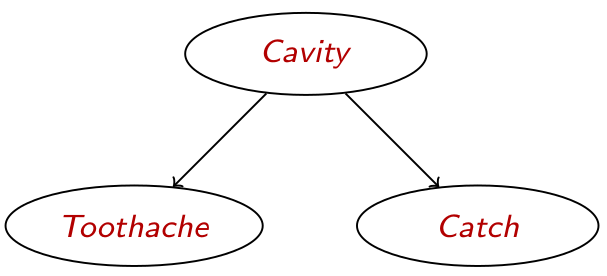
\includegraphics[width=0.5\textwidth]{img/img1.png}
    \end{center}
\end{example}
\begin{definition}
    The full joint distribution can be written as: \vspace{3.5pt}

    \begin{center}
        $\mathbf{P}(Cause, Effect_1, Effect_2, ..., Effect_n) = \mathbf{P}(Cause)\prod_i\mathbf{P}(Effect_i|Cause)$
    \end{center} \vspace{3.5pt}

    This probability distribution is called \textbf{Naive Bayes}\footnote{The naive Bayes model is the most common way to solve labeling tasks, such as classification. The total number of parameters grows \textbf{linearly}.}.
\end{definition}